\section{Leveraging Heterogeneous Approximation to Accelerate Distribute Training}
In this section we describe the different approximation modes which we explored in the course of the project. We focus on \textit{training update elisions}, which involves not updating the weights and biases of specific layers at certain training steps. Two kinds of training elisions were explored:
\begin{itemize}
	\item \textit{Selective Training Elision} involves training the entire network until a given training step $\kappa$. For steps succedding $\kappa$, only parameters corresponding to certain layers are updated, while updates for other layers are elided.
	\item \textit{Periodic Training Elision} involves performing training elisions once every $n$ steps, where $n$ is called the periodic elision interval. The parameters of the entire network are updated for $n-1$ steps, followed by a step where only parameters corresponding to certain layers are updated.
\end{itemize}

Both types of approximations partially update the model weights in a specified training step. We expect that using update elision will  reduces the amount of computation required in a training step, as well as the communication overhead required for distributed training. 

\subsection{Results}
We now discuss the experimental results. Different approximation techniques are compared on the basis of classification accuracy (on held out data) and training time. We present results for both single node training as well as distributed training for a number of different cluster configurations. In each of our experiments, we checkpoint the model every 1000 trained steps, and use the checkpointed model to compute the achieved classification accuracy.

\subsubsection{Single Node Training}
\begin{figure}[t]
	\centering
	\includegraphics[width=0.8\columnwidth]{figures/approx.eps}
	\caption{Selective Training Elision (after 5000 steps)}
	\label{fig:approx}
\end{figure}

In Figure \ref{fig:approx}, we plot the obtained accuracy versus the training step for a selective training elision experiment running on a single machine. For each of the compared experiments we train all layers of the model until the 5000th training step. For the subsequent steps the training data is used to update only the top $\eta$ trainable layers of the model, where $\eta$ was chosen between $1$ to $4$ in our experiments. Note that, for a $N$ layer neural network $\eta=i$ corresponds to update elision for the first $N-\eta$ trainable layers. From the plot we can observe that eliding layer updates has a slight impact on accuracy. The fewer the number of elided layers, the greater the accuracy of the trained model. 

\begin{figure}[t]
	\centering
	\includegraphics[width=0.8\columnwidth]{figures/periodic-approx-2.eps}
	\caption{Periodic Selective Training Elision (every 2 steps)}
	\label{fig:periodic-approx-2}
\end{figure}
\begin{figure}[t]
	\centering
	\includegraphics[width=0.8\columnwidth]{figures/periodic-approx-5.eps}
	\caption{Periodic Selective Training Elision (every 5 steps)}
	\label{fig:periodic-approx-5}
\end{figure}

In Figures \ref{fig:periodic-approx-2} and \ref{fig:periodic-approx-5}, we plot the obtained accuracy versus the training step for periodic selective training elision experiments running on a single machine. For the experiments shown in Figure \ref{fig:periodic-approx-2}, the periodic elision interval $n$ was set to 2, and the those in Figure \ref{fig:periodic-approx-5}, $n$ was set to 5. 

\subsection{Distributed Training}




\begin{figure}[t]
	\centering
	\includegraphics[width=0.8\columnwidth]{figures/approx-2workers.eps}
	\caption{Selective Training Elision (after 5000 steps) using 2 Asynchronous Workers}
	\label{fig:approx-2-workers}
\end{figure}

\begin{figure}[t]
	\centering
	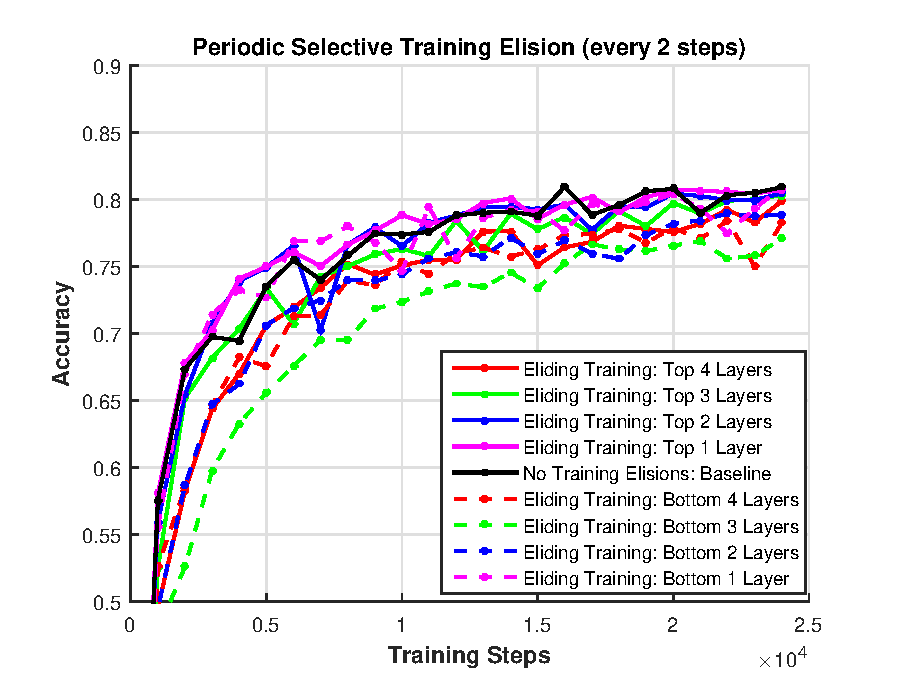
\includegraphics[width=0.8\columnwidth]{figures/combined_bottom_top_elisions.eps}
	\caption{Selective Training Elision (every 2 steps)}
	\label{fig:combined-alt}
\end{figure}
\subsection{Evaluation and Analysis}
